% preambolo per doppia compilazione HTML/PDF
\ifx\pdfoutput\undefined      % compilazione htlatex
\documentclass{article}
\DeclareGraphicsExtensions{.png, .gif, .jpg}
\newcommand{\href}[2]{\Link[#1]{}{} #2 \EndLink}
\newcommand{\hypertarget}[2]{\Link[]{}{#1} #2 \EndLink}
\newcommand{\hyperlink}[2]{\Link[]{#1}{} #2 \EndLink}
\else                         % compilazione pdflatex
\documentclass{article}
\usepackage{graphicx}
\usepackage{listings}
\usepackage{fancyhdr}
\usepackage{wrapfig}
\usepackage{multirow}
\usepackage{lscape}
\usepackage{amssymb,amsmath}
\pdfpagewidth 8.5in
\pdfpageheight 11in
\setlength\textwidth{5.7in}
\setlength\textheight{8.1in}
\setlength\oddsidemargin{0in}
\setlength\evensidemargin{0in}
\setlength\topmargin{-0.6in}
\setlength\footskip{0.6in}
\setlength\headsep{0.6in}
\usepackage[hyperindex]{hyperref}
\newcommand{\percent}{\,^0\!/_0}
 \hypersetup{
    bookmarks=true,         % show bookmarks bar?
    unicode=true,             % non-Latin characters in Acrobat’s bookmarks
    pdftoolbar=false,        % show Acrobat’s toolbar?
    pdfmenubar=false,      % show Acrobat’s menu?
    pdffitwindow=false,    % page fit to window when opened
    pdfauthor={Maurizio}, % author
    pdfsubject={Ungaro},  % subject of the document
    pdfnewwindow=true,   % links in new window
    colorlinks=true,           % false: boxed links; true: colored links
    linkcolor=black,           % color of internal links
    citecolor=blue,            % color of links to bibliography
    filecolor=magenta,      % color of file links
    urlcolor=blue              % color of external links
}
\fi

\begin{document}

\title{Low-Threshold Cherenkov Counter Operations Manual}

\vskip 1cm

\author{M. Ungaro, Jefferson Laboratory\\[0.2ex]
{\it ltcc\_manual.tex -- v1.0}}

\date \today
%
\maketitle

\begin{abstract}
This document provides an overview of the CLAS12 Low-Threshold Cherenkov Counter (LTCC) and serves 
as an Operations Manual for the detector. Instructions are provided for shift workers related to 
basic steps of operating and monitoring the HV controls, monitoring the detector system and 
responding to alarms, and knowing when to contact the on-call personnel. 

%More complete details 
%are also provided for LTCC system experts regarding the channel mapping to the readout electronics, 
%the cable connections and routing in Hall~B, higher-order high voltage system operations, and 
%detector servicing. 
%
%This document also provides references to the available LTCC documentation and 
%a list of personnel authorized to perform LTCC system repairs and modify system settings.

\end{abstract}

\thispagestyle{empty}


\tableofcontents

\clearpage

\section{LTCC Overview}
\label{intro}

The CLAS12 spectrometer is built around a six-coil superconducting toroidal magnet that divides the 
active detection area into six 60$^\circ$-wide azimuthal sectors. 
The spectrometer detects particles between $\sim 5$ and $\sim 40$ degrees in the Forward Detector system, and
between $\sim 40$ and $\sim 120$ degrees in the Central Detector system.

The LTCC is part of the CLAS12 Forward Detector (see Fig.~\ref{fig:ltccSectors}) and it is used for  pion/kaon discrimination. 
The LTCC consists of 6 identical sectors of lightweight mirrors, light collecting cones, 5" PMTs and magnetic shields. 
The sectors are filled with $C_4F_{10}$ gas, providing pion/kaon discrimination from 3.5 to 9 GeV/c. 
Each sector contains:

\begin{itemize}
\item 108 lightweight mirrors
\item  36 Winston Cones
\item  36 5" PMT
\item  36 magnetic shields 
\end{itemize}

\begin{figure}[ht]
  \centering
		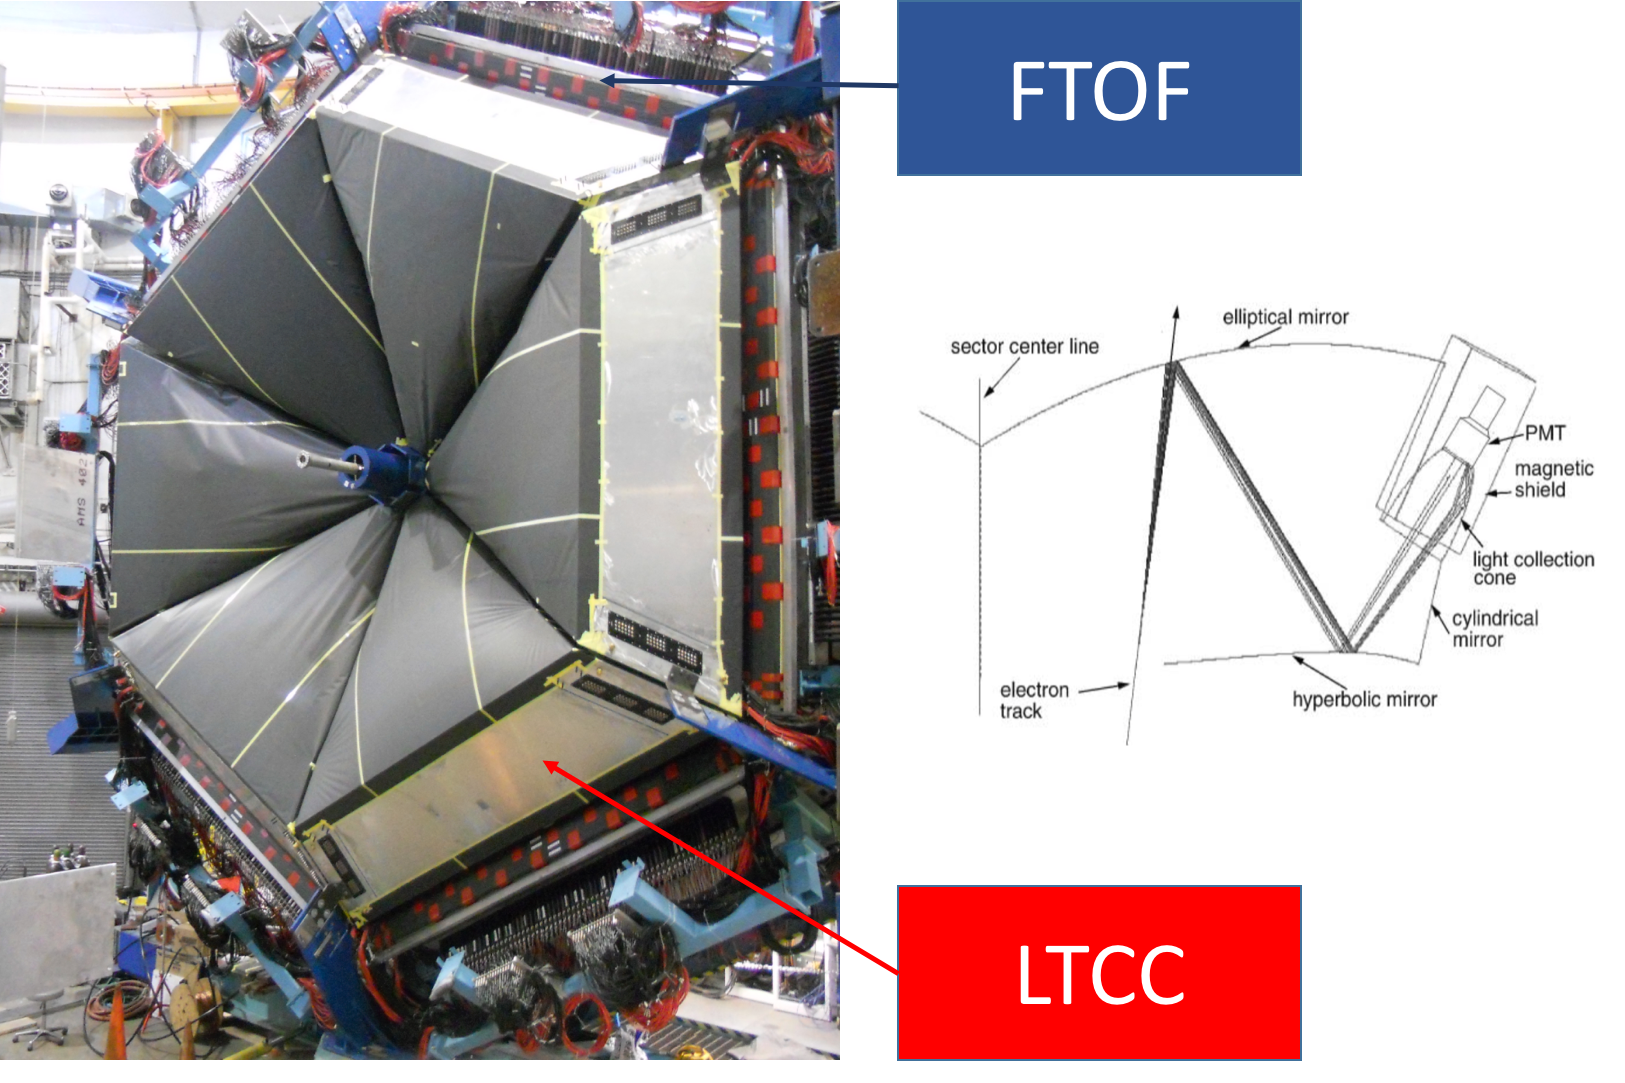
\includegraphics[width=0.98\textwidth]{img/ltccSectors}
		\caption{	Left: The LTCC sectors installed on the Forward Carriage. 
		The Forward Carriage is roughly 10 m in diameter.
		Right: The path of Cherenkov photons to the PMTs.}
 		\label{fig:ltccSectors}
\end{figure}

\clearpage

Fig.~\ref{fig:readout} shows the sector naming conventions for the LTCC system, 
as well as the definitions of the left and right sides of each sector, a block diagram of the readout electronics 
for each PMT and the rack locations for the LTCC VME electronics and HV mainframes.
Note that ``South'' refers to beam left and ``North'' to beam right (closer to the Pie Tower). 

The HV power supplies for each LTCC sector are  CAEN 1527P mainframes 
outfitted with positive polarity 24-channel A1535P modules. 
Each PMT provides two identical outputs. One is connected to JLab 
250~MHz VME flash ADCs (FADC) and the other to JLab VME leading edge discriminators and 
CAEN VME TDCs (100~ps LSB CAEN 1190A).


A summary of the LTCC technical parameters is given in Table 1.

\vspace{1cm}


\begin{table}[htbp]
\begin{center}
\begin{tabular} {|l|l|} \hline
~~Parameter~~ &~~~~~~~~~~~~~~~~~~~~~~ Design Value ~~~~~~~~~~\\ \hline \hline
\multicolumn{2}{|l|} {\bf Mirrors} \\ \hline
Support Structure    & 3 Kevlar layers sandwiched with vinyl foam  \\ \hline
Elliptical                   &  Length = 6" to 55", Width = 8" to 11"\\ \hline
Hyperbolic              & Length = 12" to 30", Width = 8" to 9.25" \\ \hline
Mirror Coating         &  $Al/MgF_2$ \\ \hline
Reflectivity             & 90\% from 250 to 650 nm  \\ \hline
\multicolumn{2}{|l|} {\bf $C_4F_{10}$  gas} \\ \hline
   Refraction Index    & 1.00134  \\ \hline
    Transparency      &  100\% above 220 nm \\ \hline
    Density               &  9.94 $Kg/m^3$ \\ \hline
     Window Material &  Tedlar/Mylar/Tedlar composite \\ \hline
\multicolumn{2}{|l|} {\bf PMTs} \\ \hline
   200  &  Photonis XP 4500B   \\ \hline
    16   &  Photonis XP 4500 (Quartz Window) \\ \hline
\multicolumn{2}{|l|} {\bf Magnetic Shields} \\ \hline
    Material                         &  Eagle AAA: 80\% Ni, 4.20\% Mo, and 15\% Fe \\ \hline
    Field Attenuation Factor &  85 Axial, 390 Transverse \\ \hline
\multicolumn{2}{|l|} {\bf PID} \\ \hline
    $\pi / K$ separation &  3.5 to 9 GeV/c\\ \hline
\end{tabular}
\caption{Table of parameters for the LTCC mirrors, gas, PMTs, and their shielding.}
\label{details}
\end{center}
\end{table}


\clearpage

\begin{figure}[ht]
  \centering
		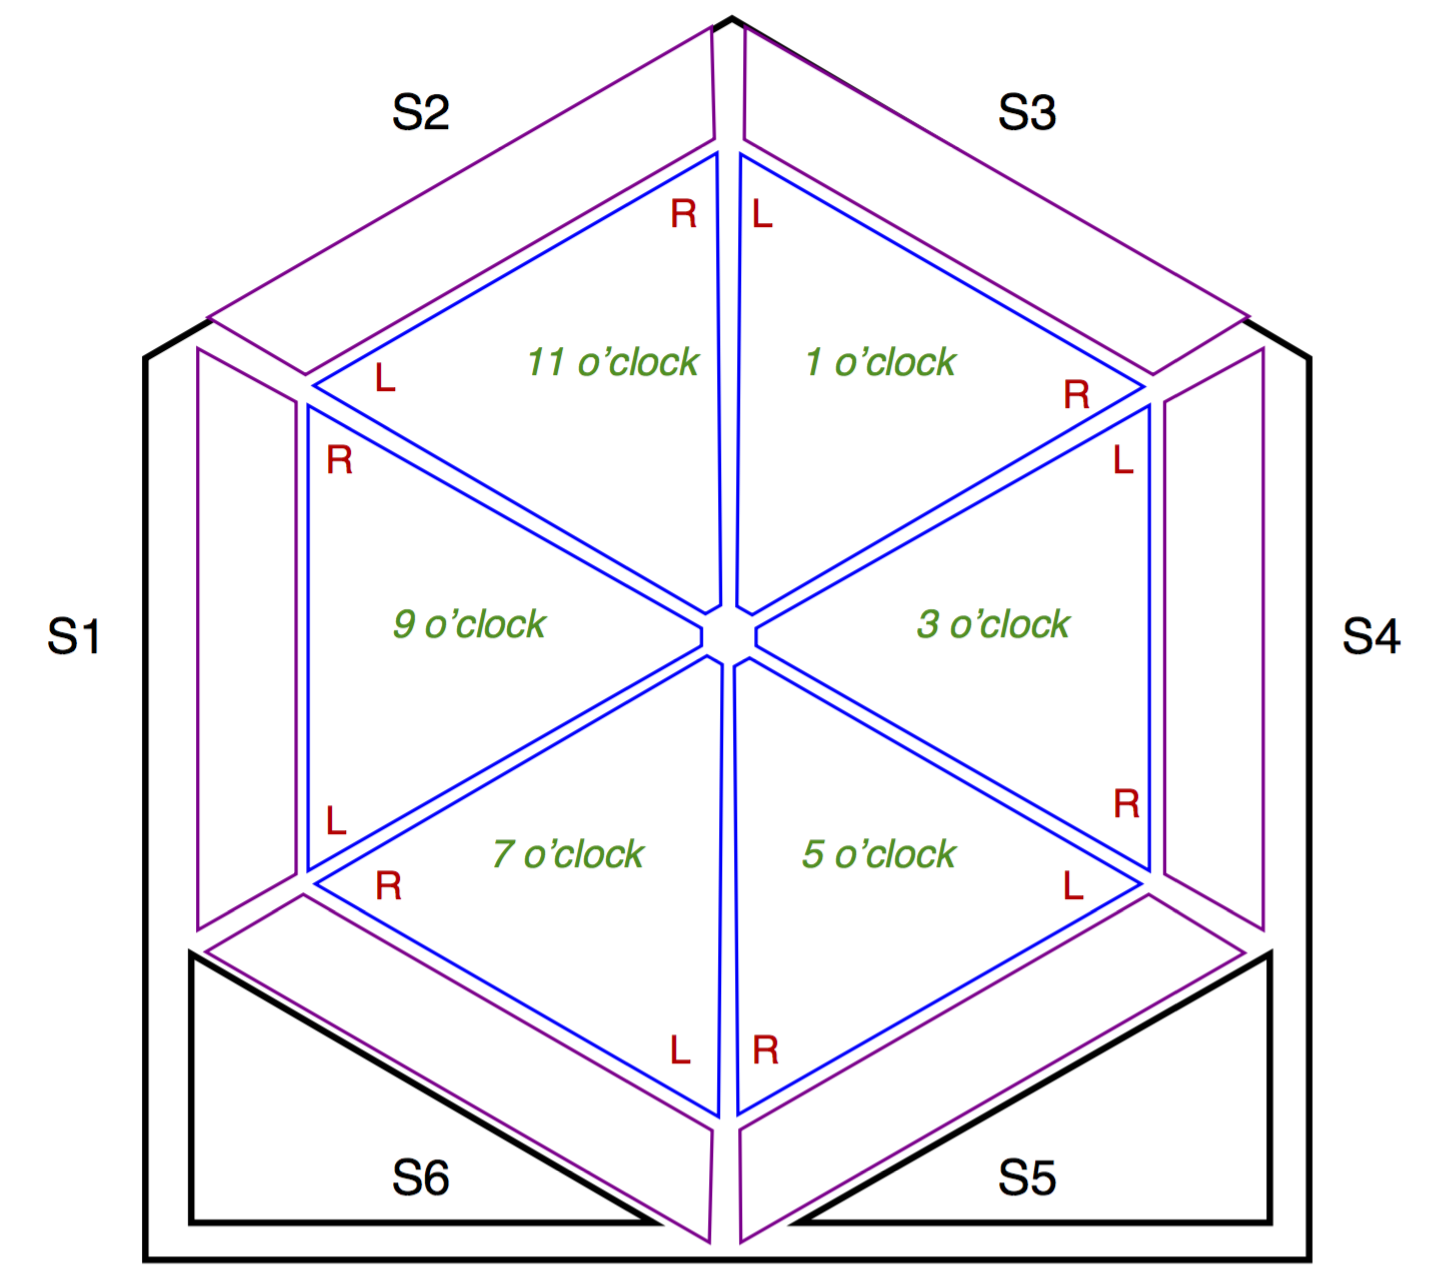
\includegraphics[width=0.8\textwidth]{img/sectorScheme} \\
		\vspace{1cm}
		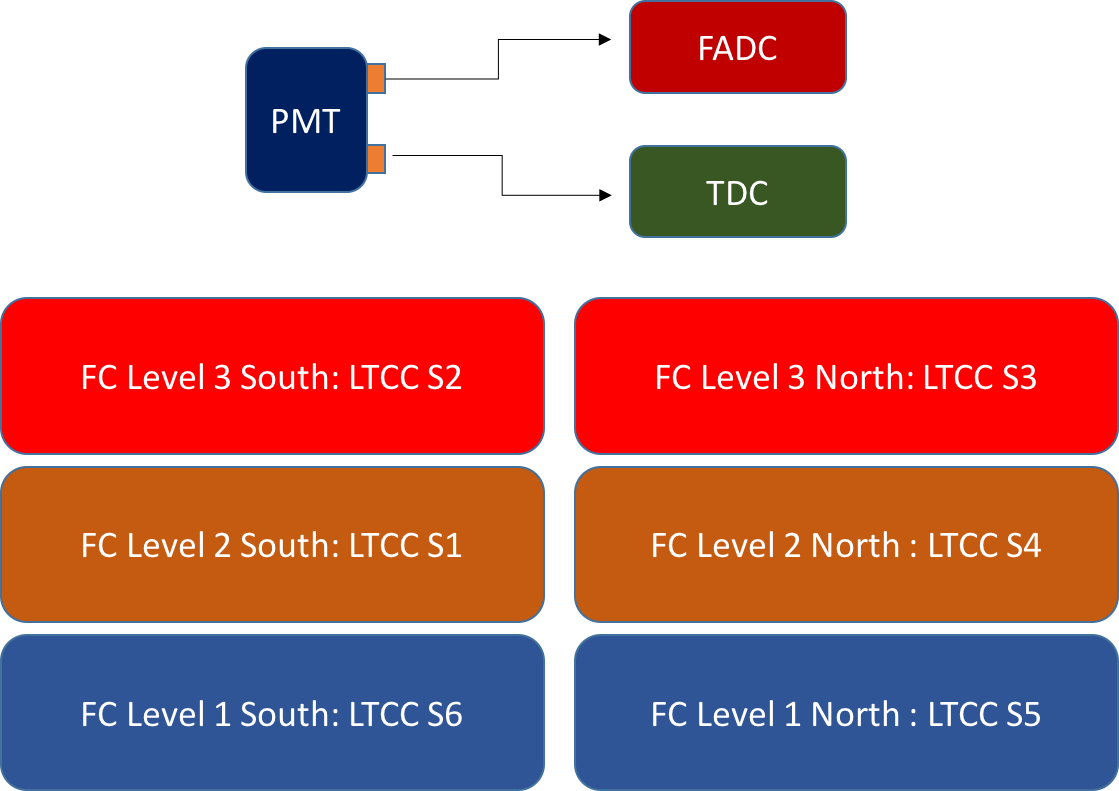
\includegraphics[width=0.8\textwidth]{img/readout}
		\caption{LTCC naming conventions and readout system.  Top: each PMT connects two identical outputs to both FADC and TDC. 
		 Bottom: the location of the HV and readout electronics for each sector. }
 		\label{fig:readout}
\end{figure}



\clearpage



\section{Information for Shift Workers}

\subsection{Shift Worker Responsibilities}

The shift worker in the Hall~B Counting House has five responsibilities with regard to the LTCC
system:

\begin{enumerate}
\item Updating the Hall~B electronic logbook with records of problems or system conditions (see 
Section~\ref{logbook}).

\item Contacting LTCC system on-call personnel for any problems that are discovered (see 
Section~\ref{contact}).

\item Responding to LTCC system alarms from the Hall~B alarm handler (see Section~\ref{alarms}).

\item If necessary, turning on or off the high voltage for the LTCC system using the HV control interface (see 
Section~\ref{hv-control}).

\end{enumerate}

\subsubsection{Updating the Logbook}
\label{logbook}

The electronic logbook (or e-log)~\cite{e-log} is set up to run on a specified terminal in the 
Hall~B Counting House. Shift workers are responsible for keeping an up-to-date and accurate record
of any problems or issues concerning the LTCC system. For any questions regarding the logbook, its
usage, or on what is considered to be a ``logbook worthy'' entry, consult the assigned shift leader.

\subsubsection{Contacting LTCC System Personnel}
\label{contact}

As a general rule, shift workers should spend no more than 10 to 15 minutes attempting to solve
any problem that arises with the LTCC system. At that point they should contact the assigned 
LTCC on-call worker to either provide advice on how to proceed or to address the problem.

This document is divided into a section for shift workers and LTCC system experts. However, only 
LTCC system experts (as listed in Section~\ref{personnel}) are authorized to make changes to the 
LTCC parameter settings, to work on the hardware or electronics, or to modify the DAQ system 
software. This division between shift worker responsibilities and expert responsibilities is
essential to maintain in order to protect and safeguard the equipment, to ensure data collection
is as efficient as possible, and to minimize down time. If the shift worker has any questions 
regarding how to proceed when an issue arises, the shift leader should be consulted.


\clearpage
\subsubsection{Hall~B Alarm Handler}
\label{alarms}

The BEAST alarm handler system running in the Counting House monitors the entire Hall~B Slow Controls
system. This includes HV and LV systems, gas systems, torus and solenoid controls, subsystem
environment controls (e.g. temperature, humidity), and pulser calibration systems (among several
others). The system runs on a dedicated terminal in the Counting House. One of the main responsibilities
of the shift worker is to respond to alarms from this system, either by taking corrective action
or contacting the appropriate on-call personnel. Instructions and details on the alarm handler for Hall~B
are given in Ref.~\cite{beast}.

For the LTCC system, the two elements monitored by the alarm handler are the HV and gas systems.
Any time a channel trips off an alarm will sound. The alarm handler will identify the specific
channel (or channels) that have tripped. These channels can be reset either through the alarm handler
or through the nominal LTCC HV control screens. These channels should be reset only after ensuring
that whatever condition caused the trip (e.g. bad beam conditions) has been addressed.

\subsection{High Voltage Controls}
\label{hv-control}

The LTCC HV is controlled through the Hall~B CS-Studio suite, which is an Eclipse-based collection 
of tools used as an interface to the EPICS Slow Controls system. To start the user interface on any 
terminal in the Hall~B Counting House, enter the command {\it clascss}. Fig.~\ref{fig:clascss}(left) 
shows the control panel that is launched.

\begin{figure}[ht]
  \centering
		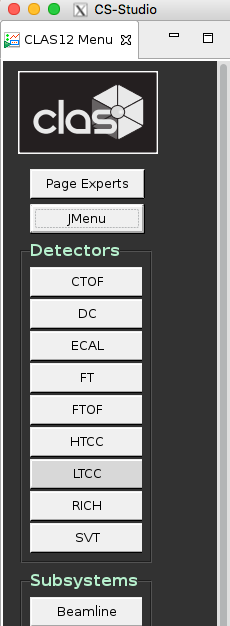
\includegraphics[width=0.22\textwidth]{img/clascss1}
		\hspace{2cm}
		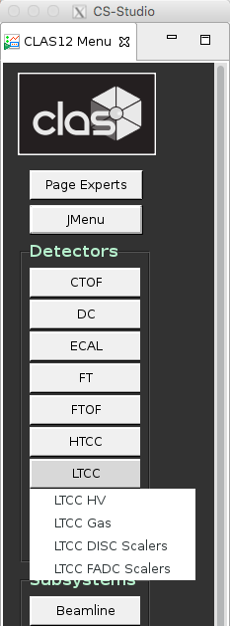
\includegraphics[width=0.22\textwidth]{img/clascss2}
	\caption{The CS-Studio interface used for the Slow Controls of the CLAS12 detectors and subsystems. 
	(Left) General CLAS12 interface. (Right) Options for the LTCC system.}
 		\label{fig:clascss}
\end{figure}

\clearpage
To bring up the LTCC HV controls, click on the ``LTCC'' button on the subsystem list. This pops up a 
sub-menu of all Slow Controls subprograms for the LTCC system 
(see Fig.~\ref{fig:clascss}(right)). Clicking the mouse on the ``LTCC HV'' option brings up the HV control 
interface for the LTCC system as shown in Fig.~\ref{fig:ltccHV}. This interface allows for HV 
operations at a number of functionality levels:

\begin{itemize}
\item All channels in the full LTCC system
\item All channels in a single LTCC sector
\item The left  or the right PMTs in a given sector
\item A single PMT in the LTCC system
\end{itemize}

\begin{figure}[ht]
  \centering
		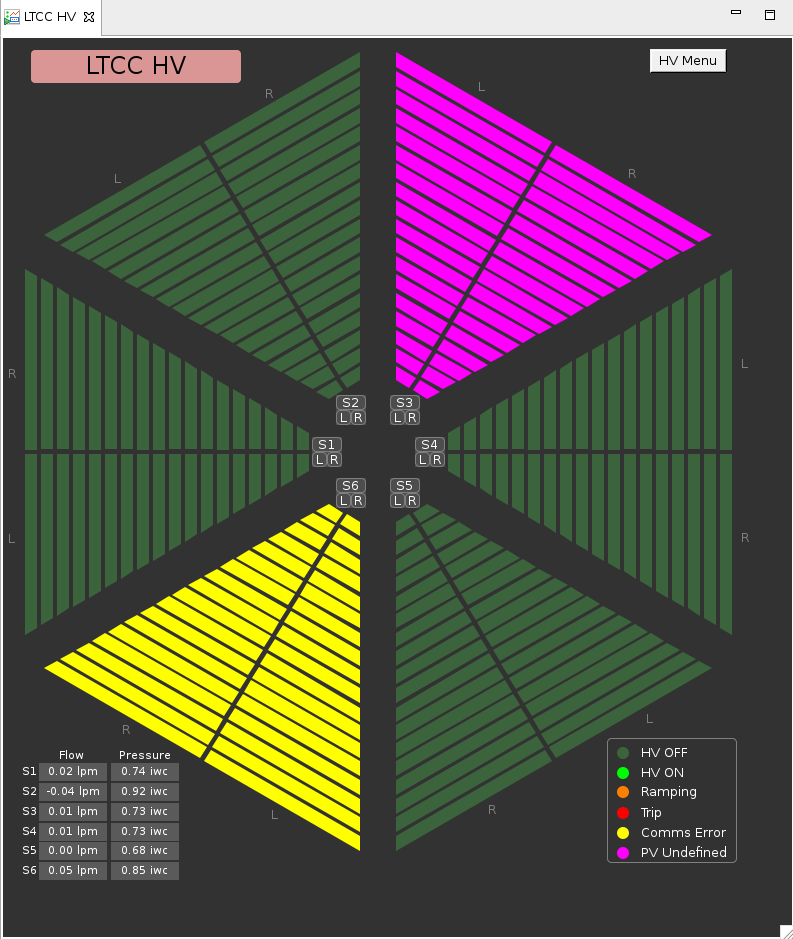
\includegraphics[width=0.81\textwidth]{img/ltccHV}
		\caption{LTCC HV display and control interface. }
 		\label{fig:ltccHV}
\end{figure}

\clearpage

For the shift worker the most common operations are:

\begin{enumerate}
\item To turn the HV for all system PMTs on or off. This is accomplished by clicking the button in the 
upper right corner ``HV MENU''. This pops up a sub-menu with the relevant options.

\item To turn the HV for all PMTs in a single sector on or off. This is accomplished by clicking on 
the corresponding sector button at its nose, denoted with the letter S followed by the sector number. This pops up a 
sub-menu with the relevant options.

\item To turn the left or right HV for the PMTs in a given  sector on or off. This is accomplished by
clicking on either the L or the R buttons near the sector nose. This pops
up a sub-menu with the relevant options as shown in Fig.~\ref{fig:ltccHVactions} (right).

\item To turn individual PMTs on or off. This is accomplished by clicking on the segment representing 
the channel of interest. Hovering on the detector picture pops up the segment nomenclature, see 
Fig.~\ref{fig:ltccHVactions} (left). Clicking on the segment  brings up a control screen for the channel of interest as shown in
Fig.~\ref{fig:singleHV}. Clicking on the ``Pw'' button toggles the channel HV on and off.

\end{enumerate}

\begin{figure}[ht]
  \centering
		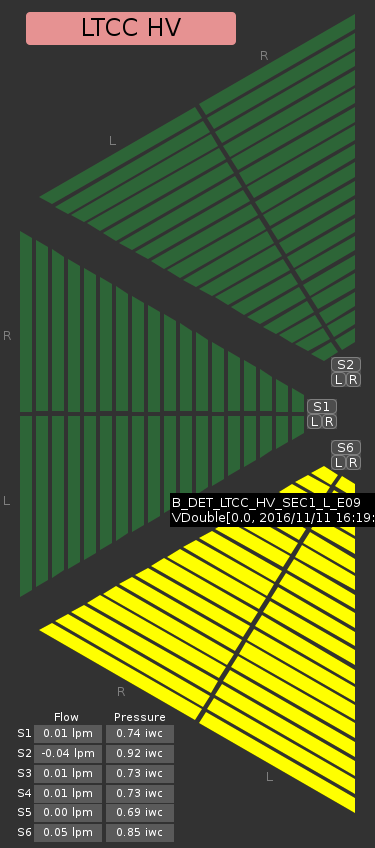
\includegraphics[width=0.33\textwidth]{img/ltccHVhover}
		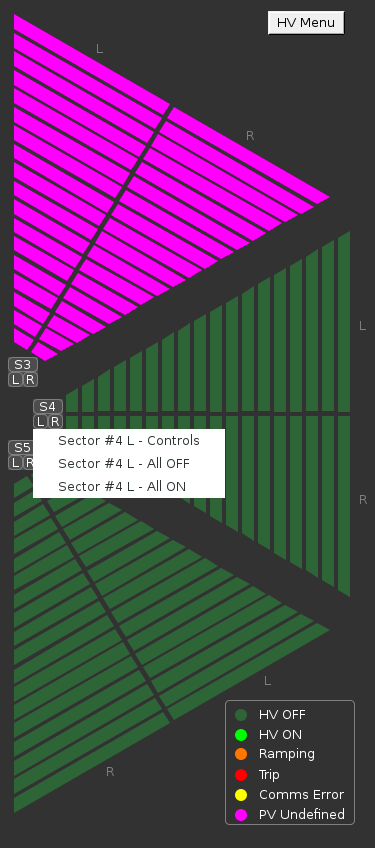
\includegraphics[width=0.33\textwidth]{img/ltccHVlr}
		\caption{	(Left) Hovering on a LTCC segment will display its index. (Right) Clicking on the L 
	button brings up options for all PMTs on the left of that sector.}
 		\label{fig:ltccHVactions}
\end{figure}

\clearpage

\begin{figure}[ht]
  \centering
		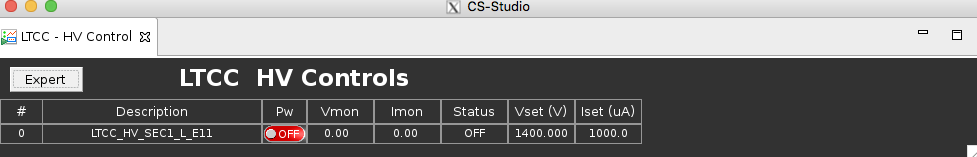
\includegraphics[width=0.98\textwidth]{img/singleHV}
		\caption{LTCC HV display and control interface  for single channel parameters..}
 		\label{fig:singleHV}
\end{figure}


If the ``Controls'' option is selected for a sector or a left/right part of a sector, a ``novice'' 
window is opened as shown in Fig.~\ref{fig:ltccHVcontrols}. This window shows the monitored channel voltage 
and current ($V_{mon}$ (V) and $I_{mon}$ ($\mu$A)), the channel status (OFF, ON), and the set channel
voltage and current ($V_{set}$ (V) and $I_{set}$ ($\mu$A)). If desired, shift workers can toggle the
HV settings for single channels on or off through this interface.


\begin{figure}[ht]
  \centering
		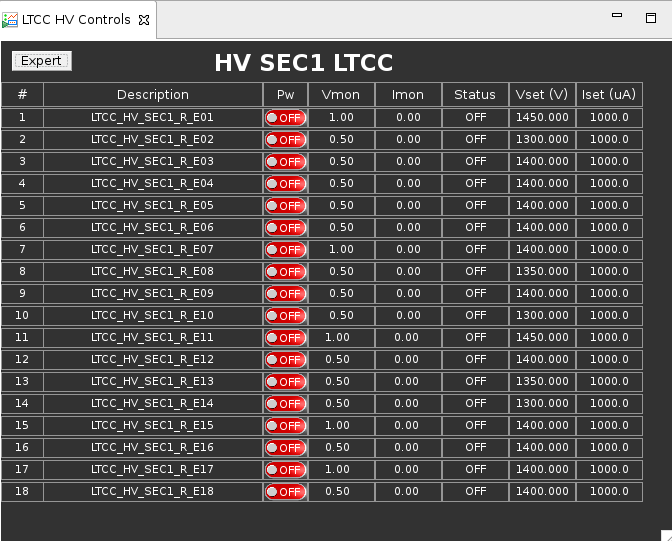
\includegraphics[width=0.82\textwidth]{img/ltccHVcontrols}
		\caption{LTCC HV “novice” channel controls screen. }
 		\label{fig:ltccHVcontrols}
\end{figure}

\clearpage

In the upper left corner of this ``Channel Controls'' window is a button marked ``expert'' that
brings up the window shown in Fig.~\ref{fig:hvcontrolsE}. This allows changes to the system settings
for the maximum channel current, maximum channel voltage setting, and the channel HV ramp up and 
ramp down rates. Clicking on the ``novice'' button in the upper left corner toggles between the 
expert and novice screens. \textcolor{red}{The expert screen should only be used by the list of 
authorized LTCC personnel given in Section~\ref{personnel}.} 

\begin{figure}[ht]
  \centering
		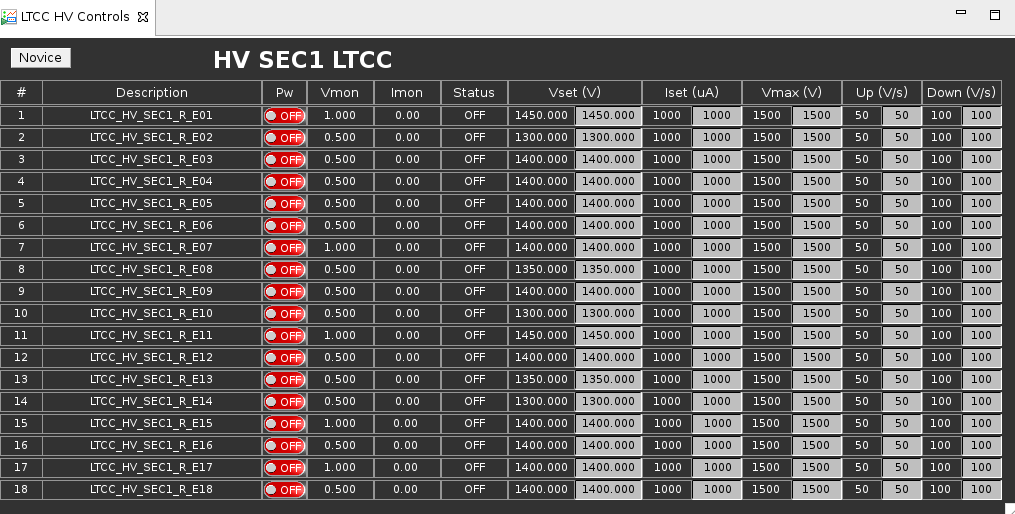
\includegraphics[width=0.92\textwidth]{img/ltccHVcontrolsExpert}
		\caption{LTCC HV  “expert” channel controls screen.}
 		\label{fig:hvcontrolsE}
\end{figure}


The HV Control Interface screen (see Fig.~\ref{fig:ltccHV}) also provides a color key to indicate 
the channel status:

\begin{itemize}
\item HV off - no highlight color (channel color dark green)
\item HV on - bright green
\item HV ramping up or ramping down - orange
\item HV trip - red
\item Communication problem - yellow
\item Undefined channel status - magenta
\end{itemize}

\clearpage

\section{Resetting the IOCs}
\label{reset-iocs}

If there is a communication problem present, which typically appears for all PMTs in a given sector,
the usual cause is an issue of communication between the IOC computer and the HV mainframe. To reboot 
the IOC for a given sector, click on ``IOCs'' button on the Slow Controls panel within the ``Subsystems'' 
portion of the interface (see Fig.~\ref{fig:clascss}). Fig.~\ref{fig:ioc} (left) shows the options that 
appear on the sub-menu that pops up. On this menu, select ``HV IOC Health'' to open the control window 
shown in Fig.~\ref{fig:ioc} (right). Click on the ``Reboot'' button for the HV supply that has the IOC 
communication problem. The reboot will take less than two minutes to complete and the yellow 
communication problem channel indicators should all disappear. If 
rebooting the IOC does not solve the problems, contact the Slow Controls system expert.

\begin{figure}[ht]
  \centering
		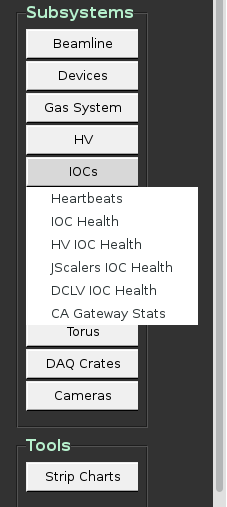
\includegraphics[width=0.20\textwidth]{img/ioc}
		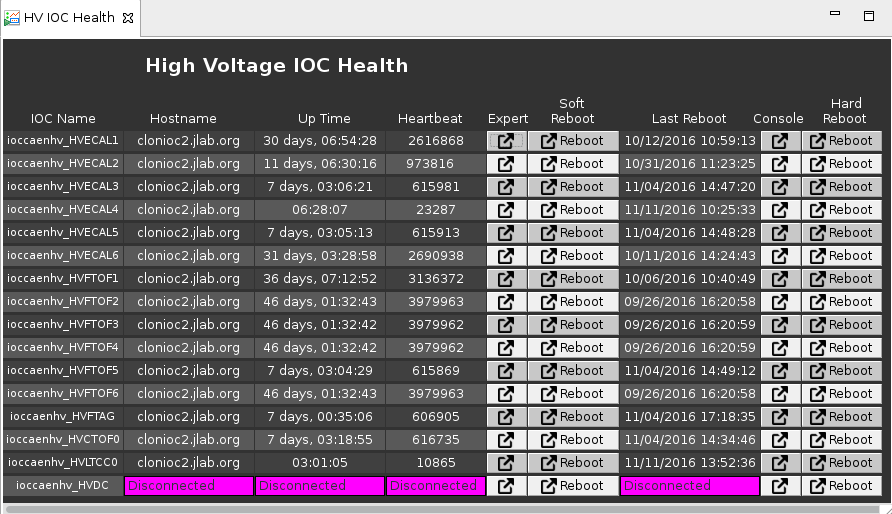
\includegraphics[width=0.77\textwidth]{img/iocHV}
		\caption{LTCC HV  “expert” channel controls screen.}
 		\label{fig:ioc}
\end{figure}

\clearpage

\section{LTCC Authorized Personnel}
\label{personnel}

Beyond turning on/off the LTCC system HV and monitoring the system scalers, all other operations and
repairs are only to be carried out by the list of authorized personnel shown in Table~\ref{expert-list}.
The list of authorized personnel for LTCC can only be modified by LTCC Group Leader.

\begin{table}[ht]
\begin{center}
\begin{tabular} {|c|c|c|c|} \hline
Name                 & Telephone         & email                    & Area             \\ \hline \hline
Maurizio Ungaro  & 757-269-7578  & ungaro@jlab.org    & LTCC Group Leader\\ \hline
Cole Smith          &                         & lcsmith@jlab.org    & Hardware         \\ \hline
Sergey Boyarinov & 757-269-5795 & boyarinov@jlab.org & DAQ              \\ \hline
George Jacobs     & 757-269-5902 & jacobsg@jlab.org    & Gas System    \\ \hline
Nathan Baltzell     & 757-269-5902 & baltzell@jlab.org     & Slow Controls    \\ \hline
\end{tabular}
\caption{LTCC detector authorized personnel.}
\label{expert-list}
\end{center}
\end{table}



\clearpage



\begin{thebibliography}{99}

\bibitem{e-log}
Hall~B Electronic Logbook: https://logbooks.jlab.org/book/hblog

\bibitem{beast}
Hall~B BEAST alarm handler: \\
https://clasweb.jlab.org/wiki/index.php/Slow\_Control\_Alarms


\end{thebibliography}

\end{document}